\section{The RootSystem class} \label{sec:rs}

The class RootSystem is responsible for the model parameter and controls the simulation.
Additionally, the class offers utility functions for post processing on a per root level. 
Post processing functions per segment can be found in the class SegmentAnalyser (see Section \ref{sec:sa}).

\subsection{Initialize parameters from scratch} \label{sec:from_scratch}
 
In the previous examples we always opened the root system parameters from a file. 
In this example we show how to do everything in a Python script without the need of any parameter files. 
This is especially important if we want to modify any of the parameters in our scripts, 
like it is needed for a sensitivity analysis in Section \ref{ssec:sensitivity}.

In order to set up a simulation by hand, we have to define all relevant model parameters. 
This is done by creating a RootRandomParameter object for each root type, and 
SeedRandomParameter for each plant type. 

Note that within the simulation, the parameters for a specific root (RootSpecificParameter) 
are generated from the RootRandomParameter that represents the random distributions of certain parameters.

\lstinputlisting[language=Python, caption=Example 2a]{../../examples/python/example2a_initialize.py}

\begin{itemize}

\item[11,12] Create the root type parameters of type 1 and type 2.
\item[16-36] We set up a simple root system by hand. 
First we define the tap root L14-L27, then the laterals L29-L36. By default all standard deviations are 0. 
Most parameters standard deviations can be set with an additional 's' appended to the parameter name, 
e.g. las is the std of la, see L32
\item[38,39] Set the root type parameters.

\item[32-46] Create the seed random parameter stating when basal and shoot borne roots emerge. 
In this example we neglect shoot borne roots, and just define the seed location and  the emergence times (in days) 
of the basal roots.
\item[47] Sets the root system parameters.

\item[49] We state the root types of basal and shoot borne roots. 
Per default these types are 4 (for basal) and 5 (for shootborne). 
If they are not set a warning is produced and the tap root type 1 is taken. 
\item[50,51] Simulate and export results. 

\item[57-55] It is not only possible to set all model parameter, 
but to retrieve all parameters after the simulation with rs.getParameter. 
For all parameters that are derived from a distribution the root specific parameters are returned (L56), 
i.e. the values that were drawn from the normal distribution. 
The root random parameter can be accessed by adding '\_mean', '\_dev' to the parameter value (L57).  

\item[56-63] Simulation results can also accessed with getParameter(), 
which returns the parameter value per root. Especially, note the difference between la, and la\_mean

\end{itemize}

Note that all parameters can be set and modified within Python. 
Especially, standard deviations can be set to zero in order to be able to precisely predict the result. 
For example we can calculate the total root system length analytically, 
and check if the numerical simulation yield the (exact) same result. 
This is performed in the tests withing test\_root.py, and test\_rootsystem, 
which is used to test and validate CPlantBox and formerly CRootBox.



\subsection{Root system length over time}

The following script shows how to analyse root system length versus time. 

\lstinputlisting[language=Python, caption=Example 3a]{../../examples/python/example2b_length.py}

\begin{itemize}

\item[6] NumPy is Python's scientific computing package.
\item[7] Matplotlib is Python's easy way to create figures like in Matlab.

\item[9-14] Sets up the simulation.

\item[16-18] Defines the simulation time, time step, and the resulting number of simulate(dt) calls. 

\item[21] First we state which scalar type we want to analyse (others are type, radius, order, time, surface, one, parenttype)

\item[22] Pre-definition of the NumPy arrays storing the lengths over time. 

\item[23-30] The simulation loops executes the simulation for a single time step L24. L25 calculates the type of each root, L26 the length (or other scalar type) of the root. L27-L30 calculates the total root length in the time step for all roots, and for specific root types.

\item[32-38] Creates Figure \ref{fig:length}.

\end{itemize}



\subsection{Root tips and root bases}

Next we show two options how to retrieve root tip postions and root base positions from a simulation:

\lstinputlisting[language=Python, caption=Example 3b]{../../examples/python/example2c_roottips.py}

\begin{itemize}

\item[14,15] Reset the simulation and simulate for only 7 days (otherwise there are so many root tips).

\item[17-18] Outputs the number of nodes and segments to get an idea how big the resulting root system is. 
Note that number of segments equals the number of nodes minus the number of base roots that will emerge. 
Base roots are tap roots, basal roots and shootborne roots.

\item[20-36] The first approach retrieves all roots as polylines L50. 
Root tips are the last nodes of the polylines L54, root bases the first nodes L53. 
Roots that have not started to grow have only 1 node, and are not retrieved by getPolylines().

\item[28-31] Second approach: L29 rs.getNodes() returns all nodes of the root system as a list of Vector3d objects. 
Each Vector3d object can be converted into a numpy array automatically, 
but is necessary to do that for each element of the list. The methods L30, L31 return the indices of the tips and bases. 

\item[33-41] Creates Figure \ref{fig:scatter} using the second approach.

\item[44,45] Verifies that both approaches yield the same result.

\end{itemize}

\begin{figure}
\begin{subfigure}[c]{0.5\textwidth}
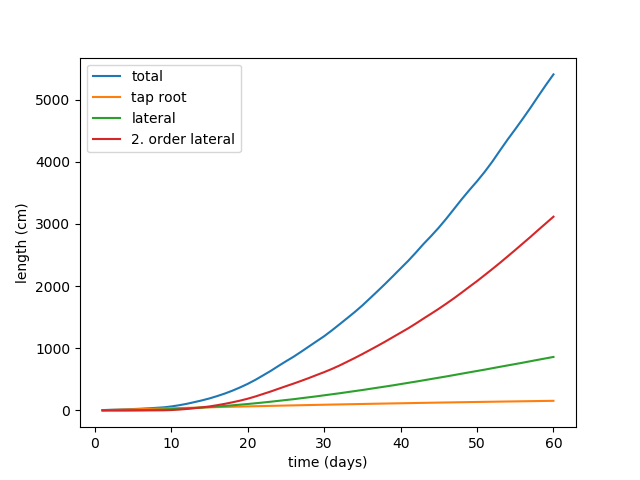
\includegraphics[width=0.99\textwidth]{example_3a.png}
\subcaption{Total root length versus time} \label{fig:length}
\end{subfigure}
\begin{subfigure}[c]{0.5\textwidth}
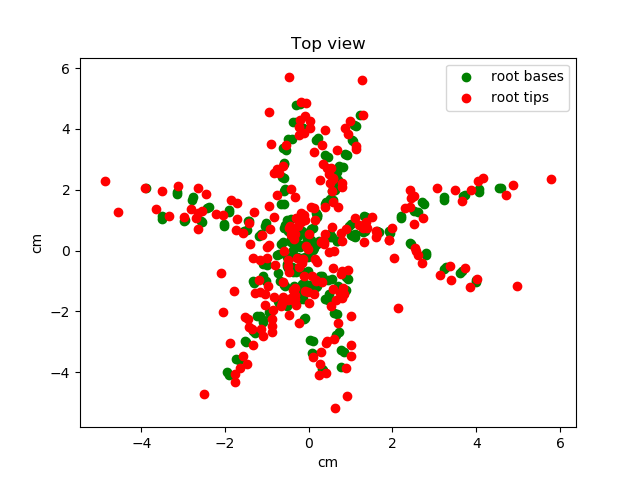
\includegraphics[width=0.99\textwidth]{example_3b.png}
\subcaption{Top view of the root tip and root bases} \label{fig:scatter}
\end{subfigure}
\caption{Root system analysis: Example 2b (a), Example 2c (b)} 
\end{figure}


